\documentclass[8pt]{amsart}
\usepackage{amsmath, amssymb}
\usepackage{amsfonts}
\usepackage{mathrsfs}
\usepackage[arrow,matrix,curve,cmtip,ps]{xy}
\usepackage{paralist}
\usepackage[left=1in,top=1in,right=1in,bottom=1in]{geometry}
\usepackage{amsthm}
\usepackage{tikz}
\usetikzlibrary{arrows,chains,matrix,positioning,scopes}

\allowdisplaybreaks

\theoremstyle{plain}% default

\theoremstyle{definition}
\newtheorem{theorem}{Theorem}[section]
\newtheorem{lemma}{Lemma}[section]
\newtheorem*{proposition}{Proposition}
\newtheorem*{corollary}{Corollary}
\newtheorem*{KL}{Klein’s Lemma}

\newtheorem*{definition}{Definition}
\newtheorem{conjecture}{Conjecture}[section]
\newtheorem{example}{Example}[section]
\newtheorem*{exercise}{Exercise}%[section]
\newtheorem*{notation}{Notation}
\newtheorem*{remark}{Remark}

\theoremstyle{remark}
\newtheorem*{note}{Note}
\newtheorem{case}{Case}

%this has equations numbered within sections 1.1,1.2, ... 2.1,...
\numberwithin{equation}{section}

\makeatletter
\newenvironment{solution}
               {\let\oldqedsymbol=\qedsymbol%
                \def\@addpunct##1{}%
                \renewcommand{\qedsymbol}{$\blacktriangleleft$}%
                \begin{proof}[\itshape Solution.]}%
               {\end{proof}%
                \renewcommand{\qedsymbol}{\oldqedsymbol}}
\makeatother

\makeatletter
\tikzset{join/.code=\tikzset{after node path={%
\ifx\tikzchainprevious\pgfutil@empty\else(\tikzchainprevious)%
edge[every join]#1(\tikzchaincurrent)\fi}}}
\makeatother

\tikzset{>=stealth',every on chain/.append style={join},
         every join/.style={->}}




\def\upint{\mathchoice%
    {\mkern13mu\overline{\vphantom{\intop}\mkern7mu}\mkern-20mu}%
    {\mkern7mu\overline{\vphantom{\intop}\mkern7mu}\mkern-14mu}%
    {\mkern7mu\overline{\vphantom{\intop}\mkern7mu}\mkern-14mu}%
    {\mkern7mu\overline{\vphantom{\intop}\mkern7mu}\mkern-14mu}%
  \int}
\def\lowint{\mkern3mu\underline{\vphantom{\intop}\mkern7mu}\mkern-10mu\int}


%-------------------------------------------
%       Begin Local Macros
%-------------------------------------------


\newcommand{\Z}{\mathbb{Z}}
\newcommand{\N}{\mathbb{N}}
\newcommand{\Q}{\mathbb{Q}}
\newcommand{\R}{\mathbb{R}}
\newcommand{\I}{\mathbb{I}}
\newcommand{\C}{\mathbb{C}}
\newcommand{\T}{\mathbb{T}}
\newcommand{\D}{\displaystyle}
\newcommand{\im}{\operatorname{im}}
\newcommand{\coker}{\operatorname{coker}}
\newcommand{\obj}{\operatorname{obj}}
\newcommand{\Hom}{\operatorname{Hom}}
\newcommand{\Mod}{\operatorname{\textbf{Mod}}}
\newcommand{\ind}{\operatorname{ind}}
\newcommand{\rank}{\operatorname{rank}}
\newcommand\mc[1]{\marginpar{\sloppy\protect\footnotesize #1}}

%-------------------------------------------
%       End Local Macros
%-------------------------------------------
\begin{document}
\title[MATH 697]{Introduction to Homological Algebra}

% \author{Robert Cardona}

\author{
	Robert Cardona %\textit{mrrobertcardona@gmail.com}
	\and
	Massy Khoshbin %\textit{massy255@gmail.com}
	\and
	Siavash Mortezavi %\textit{siavash.mortezavi@gmail.com}
}


\address{Department of Mathematics \\ California State University Long Beach}
\email{mrrobertcardona@gmail.com \and massy255@gmail.com \and siavash.mortezavi@gmail.com}

\date{\today}


\maketitle

%%%%%%%%%%%%%%%%%%%%%%%%%%%%%%%%%%%%%%%%%%%%%%%%
\setcounter{section}{-1}
\section{MATH 697 Homework Zero.Two}
%%%%%%%%%%%%%%%%%%%%%%%%%%%%%%%%%%%%%%%%%%%%%%%%


\textbf{ AM Exercise 2.1}: Show that $(\Z/m\Z) \otimes (\Z/n\Z) = 0$ if $m$ and $n$ are coprime.
	\begin{proof}
		Choose $a \otimes b \in \Z/m\Z \otimes \Z/n\Z$. Since $m$ and $n$ are coprime, there exist $s, t \in \Z$ such that $ms + nt = 1$ Observe that $$a = a \cdot 1 = a(ms + nt) = ams + ant \equiv ant \pmod m.$$ Now observe that $$a \otimes b = atn \otimes b = a \otimes nb = at \otimes 0 = 0.$$
		We have shown that any simple tensor is zero, so any finite linear combination of simple tensors is zero. Conclude $(\Z/m\Z) \otimes (\Z/n\Z) = 0$.\\
	\end{proof}

\textbf{ AM Exercise 2.2}: Let $R$ be a ring, $I$ an ideal of $R$, $M$ an $R$-module. Show that $(R/I) \otimes_RM$ is isomorphic to $M/IM$. 
	\begin{proof}
		Define $\varphi : R/I \times M \to M/IM$ by $\varphi(r + I, m) = rm + IM$, which we shall henceforth write as $\varphi(\overline{r}, m) = \overline{rm}$. Let $(\overline{r}, m) = (\overline{s}, m)$. Then $\overline{r} = \overline{s} \implies r \in \overline{s} \implies r=s+i$, some $i \in I$. Then $\varphi(\overline{r},m)=\overline{rm}=\overline{(s+i)m}=\overline{sm+im}=\overline{sm}+\overline{im}=\overline{sm}+\overline{0}=\overline{sm}=\varphi(\overline{s},m)$. Thus $\varphi$ is well-defined.\\ 
		
		Observe $\varphi(\overline{r}+\overline{s},m)=\varphi(\overline{r+s},m)=\overline{(r+s)m}=\overline{rm+sm}=\overline{rm}+\overline{sm}=\varphi(\overline{r},m)+\varphi(\overline{s},m)$. Similarly, $\varphi(\overline{r},m+n)=\varphi(\overline{r},m)+\varphi(\overline{r},n)$. Lastly, $\varphi(\overline{rs},m)=\overline{(rs)m}=\overline{r(sm)}=\varphi(\overline{r},sm)$. Thus $\varphi$ is $R$-biadditive (In fact, $\varphi$ is $R$-bilinear).\\
		
		 Now we are guaranteed a unique $R$-homomorphism $\phi : R/I \otimes_RM \rightarrow M/IM$ given by $\phi(\overline{r} \otimes m)=\overline{rm}$. Notice if we define $f : M/IM \rightarrow R/I \otimes_RM$ via $f(\overline{m})=\overline{1}\otimes m$ then $f$ is a $\Z$-homomorphism which makes $f \circ \phi$ and $\phi \circ f$ the identity map in $R/I \otimes_RM$ and $M/IM$, respectively. So $\phi$ has a two-sided inverse, hence a bijective function, and accordingly is an isomorphism when considered as an $R$-map. 
	\end{proof}
		 

\textbf{DF \S10.5 Proposition 24}: (\textit{The Short Five Lemma}) Let $\alpha, \beta, \gamma$ be homomorphisms of short exact sequences:\\

	\begin{center}
	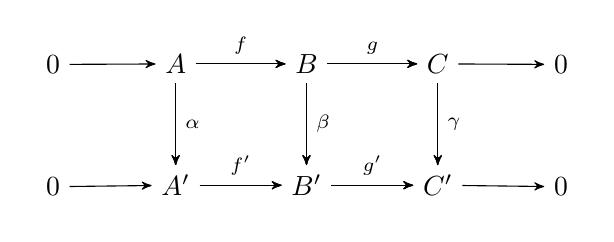
\begin{tikzpicture}
	  \matrix (m) [matrix of math nodes, row sep=3em, column sep=3em]
	    { 0 & A  & B  & C  & 0 \\
	      0 & A' & B' & C' & 0 \\ };
	  { [start chain] \chainin (m-1-1);
	    \chainin (m-1-2);
	    { [start branch=A] \chainin (m-2-2)
	        [join={node[right] {$\scriptstyle\alpha$}}];}
	    \chainin (m-1-3) [join={node[above] {$\scriptstyle f$}}];
	    { [start branch=B] \chainin (m-2-3)
	        [join={node[right] {$\scriptstyle\beta$}}];}
	    \chainin (m-1-4) [join={node[above] {$\scriptstyle g$}}];
	    { [start branch=C] \chainin (m-2-4)
	        [join={node[right] {$\scriptstyle\gamma$}}];}
	    \chainin (m-1-5); }
	  { [start chain] \chainin (m-2-1);
	    \chainin (m-2-2);
	    \chainin (m-2-3) [join={node[above] {$\scriptstyle f'$}}];
	    \chainin (m-2-4) [join={node[above] {$\scriptstyle g'$}}];
	    \chainin (m-2-5); }
	\end{tikzpicture}
	\end{center}

	\begin{enumerate}
		\item If $\alpha$ and $\gamma$ are injective then so is $\beta$.
			\begin{proof}
				Let $b \in B$ such that $\beta(b) = 0$. We want to show that $b = 0$. Observe that $g'(\beta(b)) = g'(0) = 0$. By commutativity we have $\gamma(g(b)) = g'(\beta(b)) = g'(0) = 0$. Since $\gamma$ is injective we know $g(b) = 0$ so $b \in \ker g$ but since we are in an exact sequence we have $\im f = \ker g$ and hence $b \in \im f$. By definition there exists $a \in A$ with $f(a) = b$. Now $f'(\alpha(a)) = \beta(f(a)) = \beta(b) = 0$. Since $f'$ is injective, it follows that $\alpha(a) = (f')^{-1}(0) = 0$. Now we have $a = \alpha^{-1}(0)$ and so $a = 0$. So $0 = f(a) = b$.
			\end{proof}
		\item If $\alpha$ and $\gamma$ are surjective then so is $\beta$.
			\begin{proof}
				Let $b' \in B'$ then $g'(b') \in C'$. Since $\gamma$ is surjective there excists $c \in C$ such that $\gamma(c) = g'(b')$. Since this is an exact sequence, $g$ is surjective so there exists $b \in B$ such that $g(b) = c$. By equality we have $\gamma(c) = \gamma(g(b)) = g'(b')$. Now observe that $$g'(b' - \beta(b)) = g'(b') - g'(\beta(b)) = g'(b') - \gamma(g(b)) = g'(b') - g'(b') = 0$$ So in particular $b' - \beta(b) \in \ker g'$ but by exactness $\im f' = \ker g'$ so there exists $a' \in A'$ such that $f'(a') = b' - \beta(b)$. But since $\alpha$ is surjective, there exists $a \in A$ such that $\alpha(a) = a'$. Now $f'(a') = f'(\alpha(a)) = b' - \beta(b)$. By commutativity $f'(\alpha(a)) = \beta(f(a)) = b' - \beta(b)$ so $\beta(f(a)) + \beta(b) = b'$ and we have $\beta(f(a) + b) = b'$.
			\end{proof}
		\item If $\alpha$ and $\gamma$ are isomorphisms then so is $\beta$ (and then the two sequences are isomorphism).
			\begin{proof}
				Follows from $(1)$ and $(2)$.\\
			\end{proof}
	\end{enumerate}

\textbf{R Exercise 2.14}: Let $A \xrightarrow f B \xrightarrow g C$ be a sequence of module maps. Prove that $gf = 0$ if and only if $\im f \subseteq \ker g$.  Give an example of such a sequence that is not exact.
	\begin{proof}
		Suppose $gf = 0$, that is, $f(g(a)) = 0$ for all $a \in A$. Let $b \in \im f$ then by definition there exists $a \in A$ such that $f(a) = b$. But we know by hypothesis that $0 = g(f(a)) = g(b)$ so $b \in \ker g$. Conclude that $\im f \subseteq \ker g$. Conversely, suppose that $\im f \subseteq \ker g$. Let $a \in A$ and observe that $f(a) \in \im f$. By hypothesis $f(a) \in \ker g$ so $g(f(a)) = 0$. Since $a$ was arbitrary conclude $gf = 0$.
	\end{proof}
	Consider the sequence of module maps $\Z/4\Z \xrightarrow f \Z/3\Z \xrightarrow g \Z/2\Z$ where $f(\overline x) = 2 \overline x$ and $g(\overline y) = \overline y$. Observe that $\im f = \Z/3\Z$  and $\ker g = \{0\}$. Since $\im f \neq \ker g$ it follows that this is \textbf{not} an exact sequence.\\


\textbf{R Exercise 2.15}:
	\begin{enumerate}
		\item Prove that $f : M \to N$ is surjective if and only if $\coker f = \{0\}$.
			\begin{proof}
				Suppose $f : M \to N$ is surjective then for $n \in N$, there exists $m \in M$ such that $f(m) = n$. By definition $\coker f = M/\im f = M/M = 0$. Conversely, suppose that $\coker f = 0$, i.e., $M/\im f = 0$ implying that if $m + \im f \in M/\im f$ then $m + \im f = 0$ or equivalently $m \in \im f$. Since $m$ is arbitrary, conclude $M = \im f$ and hence $f$ is surjective by definition.
			\end{proof}
		\item If $f : M \to N$ is a map, prove that there is an exact sequence $$ 0 \rightarrow \ker f \rightarrow M \xrightarrow f N \rightarrow \coker f \rightarrow 0.$$
			\begin{proof}
				Define $h : \ker f \to M$ by $h(m) = m$, that is, map each element to itself. It follows immediately that $\im h = \ker f$. Define $g : N \to \coker f = N/\im f$ by $g(n) = n + \im f$, that is, the canonical/projection mapping. Observe that $\ker g = \im f$. Conclude that the following sequence is in fact exact: $$0 \xrightarrow{\text{identity}} \ker f \xrightarrow h M \xrightarrow f N \xrightarrow g \coker f \xrightarrow{\text{zero}} 0. \qedhere$$
			\end{proof}
	\end{enumerate}

\textbf{R Exercise 2.16}:
	\begin{enumerate}
		\item If $0 \rightarrow M \rightarrow 0$ is an exact sequence, prove that $M = \{0\}$.
			\begin{proof}
				Consider $0 \xrightarrow f M \xrightarrow g 0$. Since $f$ is surjective then for $m \in M$ there exists $x \in 0$ such that $f(x) = m$ but $x$ must be $0$ so $m = 0$.
			\end{proof}
		\item If $A \xrightarrow f B \xrightarrow g C \xrightarrow h D$ is an exact sequence, prove that $f$ is surjective if and only if $h$ is injective.
			\begin{proof}
				Suppose $f$ is surjective. Then $\im f = B = \ker g$ but this immediately implies that $\im g = 0 = \ker h$ so $h$ is injective by definitoin. Conversely, suppose $h$ is injective. Then $\ker h = 0 = \im g$ which immediately implies $\ker g = B = \im f$. Conclude by definition $f$ is surjective.
			\end{proof}
		\item Let $A \xrightarrow \alpha B \xrightarrow \beta C \xrightarrow \gamma D \xrightarrow \delta E$ be exact. If $\alpha$ and $\delta$ are isomorphisms, prove that $C = \{0\}$.
			\begin{proof}
				Observe that, by previous exercise, $\beta$ is surjective and $\gamma$ is injective so we have $\im \beta = C$ and $\ker \gamma = 0$. Result follows by exactness: $C = \im \beta = \ker \gamma = 0$. Conclude $C = \{0\}$.
			\end{proof}
	\end{enumerate}



\textbf{R Exercise 2.17}: If $A \xrightarrow f B \xrightarrow g C \xrightarrow h D \xrightarrow k E$ is exact, prove that there is an exact sequence $0 \rightarrow \coker f \xrightarrow \alpha C \xrightarrow \beta \ker k \rightarrow 0$, where $\alpha : b + \im f \mapsto g(b)$ and $\beta : c \mapsto h(c)$.
	\begin{proof}
		Observe that $\ker \beta = \{c \in C : \beta(c) = h(c) = 0\} = \ker h = \im g$ by exactness and since $\alpha$ can run through any $b \in B$ conclude $\im \alpha = \im g = \ker \beta$
	\end{proof}
	
\textbf{R Exercise 2.27}: Let $V$ and $W$ be finite-dimensional vector spaces over a field $F$ and let $v_1, \dots , v_m$ and $w_1, \dots , w_n$ be bases of $V$ and $W$, respectively. Let $S:V\rightarrow V$ be a linear transformation having matrix $A=[a_{ij}]$, and let $T:W\rightarrow W$ be a linear transformation having matrix $B=[b_{kl}]$. Show that the matrix of $S\otimes T: V\otimes W\rightarrow V\otimes W$, with respect to a suitable listing of the vectors $v_i\otimes w_j$, is the $nm \times nm$ matrix $K$, which we write in block form: $$A\otimes B=\begin{bmatrix}
a_{11} B & a_{12} B & \cdots & a_{1m} B\\
a_{21} B & a_{22} B & \cdots & a_{2m} B\\
\vdots & \vdots & \ddots & \vdots \\
a_{m1} B & a_{m2} B & \cdots & a_{mm} B\\
\end{bmatrix} $$
	\begin{proof}
	Since $v_1, \dots , v_m$ is a basis for $V$ and $w_1, \dots , w_n$ is a basis for $W$, then $\{v_i\otimes w_j|1\leq i\leq m, 1\leq j\leq n\}$ is a basis for $V\otimes W$. Note that the action of $S\otimes T$ on $V\otimes W$ is induced by $S$ and $T$ on the basis vectors of $V$ and $W$, respectively: \\
	
$(S\otimes T) (v_i\otimes w_j)=S(v_i)\otimes T(w_j)$, which has the matrix representation $A(v_i)\otimes B(w_j)$. Writing $A=[a_{ij}]$ and $B=[b_{kl}]$ we have 
\begin{center}
$A(v_i)=\sum_{t=1}^ma_{it}v_t$ and $B(w_j)=\sum_{s=1}^nb_{js}w_s$.
\end{center}
Therefore $$(A\otimes B)(v_i\otimes w_j)=\sum_{t=1}^ma_{it}v_t\otimes \sum_{s=1}^nb_{js}w_s.$$ By expanding on the basis of $V$ only, we can represent $$(A\otimes B)(v_i\otimes w_j)=a_{i1}v_1\otimes B(w_j) + a_{i2}v_2\otimes B(w_j) + \cdots + a_{im}v_m\otimes B(w_j)$$ in block form as the $i$'th "row" in $A\otimes B$ times the $j$'th column basis vector of $A\otimes B$: $$\begin{bmatrix}
a_{i1} B & a_{i2} B & \cdots & a_{im} B\\
\end{bmatrix} 
\begin{bmatrix}
v_1\otimes w_j\\
v_2\otimes w_j\\
\vdots\\
v_m\otimes w_j\\
\end{bmatrix}.$$ With $1\leq i\leq m$ and $B$ being an $n\times n$ matrix, we have each "row" is an $n\times mn$ matrix. Since there are $m$ such "rows", we have that $A\otimes B$ is the $mn\times mn$ matrix as given above.
	\end{proof}

\textbf{R Exercise 2.28}: Let $R$ be a domain with $Q$ = Frac($R$), its field of fractions. If $A$ is an $R$-module, prove that every element of $Q \otimes_RA$ has the form $q \otimes a$ for $q \in Q $ and $a \in A$ (i.e. every element is a simple tensor).
	\begin{proof}
		Let $\sum_1^n q_i \otimes a_i \in Q \otimes_RA$. We can write $\sum_1^n q_i \otimes a_i = \sum_1^n \frac{r_i}{s_i} \otimes a_i$ for $r_i,s_i \in R, s_i \neq 0$. Write $s=s_1s_2\cdots s_n$ and $\widehat{s_i}=\frac{s}{s_i}$. Then $\sum_1^n \frac{r_i}{s_i} \otimes a_i = \sum_1^n (1 \cdot \frac{r_i}{s_i}) \otimes a_i = \sum_1^n (\frac{\widehat{s_i}}{\widehat{s_i}} \cdot \frac{r_i}{s_i}) \otimes a_i = \sum_1^n \frac{\widehat{s_i}r_i}{s} \otimes a_i = \sum_1^n (\frac{1}{s})\widehat{s_i}r_i \otimes a_i = \sum_1^n \frac{1}{s} \otimes (\widehat{s_i}r_i)a_i = \frac{1}{s} \otimes (\sum_1^n \widehat{s_i}r_ia_i)$.\\
	\end{proof}
	
	\textbf{R Exercise 2.29}:\textbf{(i)} Let $p$ be a prime, and let $p,q$ be relatively prime. Prove that if $A$ is a $p$-primary group and $a \in A$, then there exists $x \in A$ with $qx=a$. \\

\indent \textbf{(ii)} If $D$ is a finite cyclic group of order $m$, prove that $D/nD$ is a cyclic group of order $d=(m,n)$. \\

\indent \textbf{(iii)} Let $m$ and $n$ be positive integers, and let $d =(m,n)$. Prove that there is an isomorphism of abelian groups $$\Z_m \otimes \Z_n \cong \Z_d.$$ \\
\indent \textbf{(iv)} Let $G$ and $H$ be finitely generated abelian groups, so that \\

	\begin{center}
$G=A_1 \oplus \cdots \oplus A_n$ and $H=B_1 \oplus \cdots \oplus B_m,$  \\
	\end{center} 
	
where $A_i$ and $B_j$ are cyclic groups. Compute $G \otimes_{\Z}H$ explicitely. 
\begin{proof}
(i) $a \in A$ so $p^ka=0$, some $k \in \Z^+$. Since $p$ is prime, $(q,p)=1 \implies (q,p^k)=1$. So there exist $m,n \in \Z$ such that $qm+np^k=1$. Now $a=1\cdot a=(qm+np^k)a=qma+np^ka=q(ma)+n(p^ka)=qx+0=qx$. Observe $p^kx=p^k(ma)=m(p^ka)=0$ so $x\in A$.\\

(ii) $D$ is cyclic, so $D/nD$ is cyclic. If we write $D=<a>$, then $nD =<na>$. This is because for any $nb \in nD$, we can write $b=ka$, some $k\in \Z^+$, since $a$ generates $D$. Now $nb=n(ka)=k(na)$, and we have that $na$ generates $nD$. \\

Claim $|na|=\frac{m}{d}$. Observe $\frac{m}{d}(na)=\frac{n}{d}(ma)=\frac{n}{d}\cdot 0=0$, which implies $|na|$ divides $\frac{m}{d}$. On the other hand, if $k(na)=0$, then $(kn)a=0 \implies m|kn \implies \frac{m}{d}|k\frac{n}{d}$. But $\frac{m}{d}$ and $\frac{n}{d}$ are relatively prime by construction, forcing $\frac{m}{d}|k$. In particular, we have $\frac{m}{d}$ divides $|na|$. Thus $|na|=d$. Now $|nD|=|<na>|=|na|=\frac{m}{d}$. Lagrange's theorem gives us $|\frac{D}{nD}|=\frac{|D|}{|nD|}=\frac{m}{\frac{m}{d}}=d$. \\

(iii) By Proposition 2.68, we have that $\Z_m \otimes \Z_n \cong \Z_m/n\Z_m$. But by part (ii), $\Z_m/n\Z_m$ is a cyclic group of order $d=(m,n)$ so $\Z_m/n\Z_m \cong \Z_d$.\\

(iv) There are three cases: If both $A_i$ and $B_j$ are finite, then by part (iii) we have $A_i \otimes_\Z B_j \cong \Z_{s_i} \otimes \Z_{t_j} \cong \Z_{(s_i, t_j)}$, where $\vert A_i \vert = s_i$ and $\vert B_j \vert = t_i$. If both $A_i$ and $B_j$ are infinite, then $A_i \otimes_\Z B_j \cong \Z \otimes \Z \cong \Z$ by Proposition 2.58. If (wlog) $A_i$ is finite and $B_j$ is infinite, then $A_i \otimes_\Z B_j \cong Z_{s_i} \otimes \Z \cong \Z_{s_i}$ by Proposition 2.58. Thus we have $$G \otimes_\Z H = \D \sum_{i, j} A_i \otimes_\Z B_j = \sum_{i, j : A_i \text{ and } B_j \text{ finite}} \Z_{(s_i, t_i)} + \sum_{i, j : A_i \text{ finite and } B_j \text{ infinite}} \Z_{s_i}+ \sum_{i, j : A_i \text{ or } B_j \text{ infinite}}\Z.$$

\end{proof}


\textbf{R Exercise 2.32}: (\textit{$3 \times 3$ Lemma}) Consider the following commutative diagram in $_R\Mod$ having exact columns.
	\begin{center}
	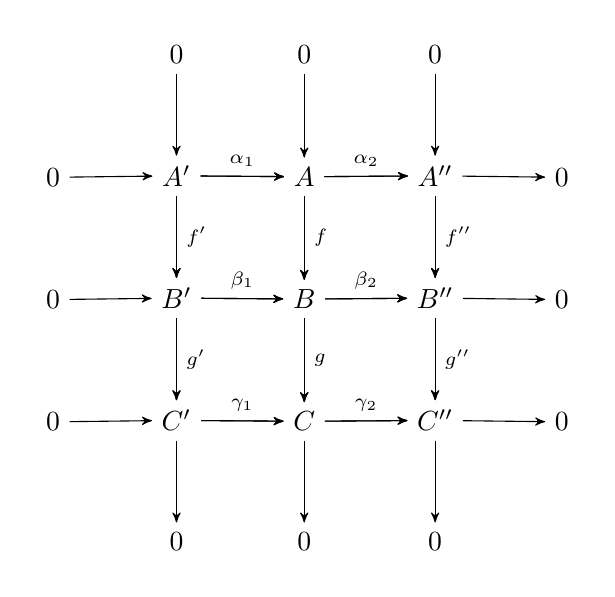
\begin{tikzpicture}

	\matrix (m) [matrix of math nodes, row sep=3em, column sep=3em]
	  {  & 0  & 0 & 0   & \\
	   0 & A' & A & A'' & 0\\
	   0 & B' & B & B'' & 0\\
	   0 & C' & C & C'' & 0\\
	     & 0  & 0 & 0   & \\};
	{ [start chain] \chainin (m-1-2); { [start branch = A] \chainin (m-2-2); } }
	{ [start chain] \chainin (m-1-3); { [start branch = B] \chainin (m-2-3); } }
	{ [start chain] \chainin (m-1-4); { [start branch = C] \chainin (m-2-4); } }
	{ [start chain] 
		\chainin (m-2-1);
		\chainin (m-2-2); 
			{ [start branch = D] \chainin (m-3-2) [join = {node[right] {$\scriptstyle f'$}}]; } 
		\chainin (m-2-3) [join = {node[above] {$\scriptstyle \alpha_1$}}];
			{ [start branch = E] \chainin (m-3-3) [join = {node[right] {$\scriptstyle f$}}]; }
		\chainin (m-2-4) [join = {node[above] {$\scriptstyle \alpha_2$}}];
			{ [start branch = F] \chainin (m-3-4) [join = {node[right] {$\scriptstyle f''$}}]; }
		\chainin (m-2-5);
	}
	{ [start chain] 
		\chainin (m-3-1);
		\chainin (m-3-2); 
			{ [start branch = G] \chainin (m-4-2) [join = {node[right] {$\scriptstyle g'$}}]; } 
		\chainin (m-3-3) [join = {node[above] {$\scriptstyle \beta_1$}}];
			{ [start branch = H] \chainin (m-4-3) [join = {node[right] {$\scriptstyle g$}}]; }
		\chainin (m-3-4) [join = {node[above] {$\scriptstyle \beta_2$}}];
			{ [start branch = I] \chainin (m-4-4) [join = {node[right] {$\scriptstyle g''$}}]; }
		\chainin (m-3-5);
	}
	{ [start chain] 
		\chainin (m-4-1);
		\chainin (m-4-2); 
			{ [start branch = J] \chainin (m-5-2); } 
		\chainin (m-4-3) [join = {node[above] {$\scriptstyle \gamma_1$}}];
			{ [start branch = K] \chainin (m-5-3); }
		\chainin (m-4-4) [join = {node[above] {$\scriptstyle \gamma_2$}}];
			{ [start branch = L] \chainin (m-5-4); }
		\chainin (m-4-5);
	}	
	\end{tikzpicture}
	\end{center}

	If the bottom two rows are exact, prove that the top row is exact; if the top two rows are exact, prove that the bottom row is exact.

	\begin{proof}
		Suppose that the bottom two rows are exact. We must show four things:
		\begin{enumerate}
			\item $\alpha_1$ is injective: Suppose $a' \in A'$ with $\alpha_1(a') = 0$. Observe that by commutativity $f(\alpha_1(a')) = \beta_1(f'(a')) = 0$ so since $\beta_1$ is injective, by exactness of the second row, $f'(a') = 0$. But since the first column is exact by hypothesis, we have $a' = 0$. Conclude that $\alpha_1$ is in fact injective.
			\item $\im \alpha_1 \subseteq \ker \alpha_2$: Choose $a \in \im \alpha_1$ then by definition there exists $a' \in A'$ such that $\alpha_1(a') = a$. Observe that $f(a) = f(\alpha_1(a')) = \beta_1(f'(a'))$ by commutativity. Moreover $\beta_2(f(a)) = f''(\alpha_2(a))$ again by commutativity. Hence we have $$\beta_2(f(a)) = \beta_2(\beta_1(f'(a'))) = 0 = f''(\alpha_2(a)).$$ Since $f''$ is injective by exactness of the third column, $\alpha_2(a) = 0$ and so $a \in \ker \alpha_2$. Conclude that $\im \alpha_2 \subseteq \ker \alpha_2$ as desired.
			\item $\ker \alpha_2 \subseteq \im \alpha_1$: Let $a \in \ker \alpha_2$ then by definition $\alpha_2(a) = 0$ and so $f''(\alpha(a)) = \beta_2(f(a)) = 0$. So $f(a) \in \ker \beta_2 = \im \beta_1$ by exactness of the second column, so there exists $b' \in B'$ such that $\beta_1(b') = f(a)$. Now $$\gamma_1(g'(b)) = g(\beta_1(b')) = g(f(a)) = 0$$ by commutativity and exactness so there exists $a' \in A'$ such that $f'(a') = b'$. Now by commutativity $$f(\alpha_1(a')) = \beta_1(f'(a')) = \beta_1(b') = f(a)$$ and so $f(a - \alpha_1(a')) = 0$ since $f$ is a homomorphism. $f$ is injective since the second column is exact so it follows that $\alpha_1(a') = a$ and so $a \in \im \alpha_1$. Conclude that $\ker \alpha_2 \subseteq \im \alpha_1$ is in fact true.
			\item $\alpha_2$ is surjective: Choose $a'' \in A''$. Consider $f''(a'') \in B''$. Since the second row is exact $\beta_2$ is surjective so there exists $b \in B$ such that $\beta_2(b) = f''(a'')$. By commutativity $g''(\beta_1(b)) = \gamma_2(g(b))$ but by exactness of the third column $g''(\beta_2(b)) = g''(f''(a'')) = 0$. So $\gamma_2(g(b)) = 0$ which implies that $g(b) \in \ker \gamma_2 = \im \gamma_1$ by exactness of the third row. So there exists $c' \in C'$ such that $\gamma_1(c') = g(b)$. Since the first column is exact $g'$ is surjective so there exists $b' \in B'$ such that $g'(b') = c'$. So $\gamma_1(c') = \gamma_1(g'(b')) = g(\beta_1(b'))$. Observe that $$g(b - \beta_1(b')) = g(b) - g(\beta_1(b')) = 0$$ since $g(b) = \gamma_1(c)$ and $g(\beta_1(b')) = \gamma_1(c)$ also. So $b - \beta_1(b') \in \ker g = \im f$ by exactness of the second column. So there exists $a \in A$ such that $f(a) = b - \beta_2(b')$. Now since $f''(\alpha(a)) = \beta_2(f(a)) = \beta_2(b - \beta_1(b'))$ we get $$f''(\alpha_2(a)) = \beta_2(b) - \beta_2(\beta_1(b')) = \beta_2(b) = f''(a'').$$ In particular we get $f''(\alpha_2(a) - a'') = 0$ but $f''$ is injective by exactness of the third column so $\alpha_2(a) = a''$. Conclude that $\alpha_2$ is in fact surjective.
		\end{enumerate}
		We have shown that if the bottom two rows are exact, then the top row is exact.\\

		Suppose that the top two rows are exact. We must show four things:
		\begin{enumerate}
			\item $\gamma_1$ is injective: Suppose $c' \in C'$  with $\gamma_1(c') = 0$. Since the first column is exact, $g'$ is surjective so there exists $b' \in B'$ such that $g'(b') = c'$. Now by commutativity $$0 = \gamma_1(c') = \gamma_1(g'(b')) = g(\beta_1(b')).$$ So $\beta_1(b') \in \ker g = \im f$ since the second row is exact. So there exists $a \in A$ such that $f(a) = \beta_1(b')$. But by commutativity $$f''(\alpha_2(a)) = \beta_2(f(a)) = \beta_2(\beta_1(b')) = 0$$ so $\alpha_2(a) = 0$. Since $f''$ is injective, because the third column is exact. Now $a \in \ker \alpha_2 = \im \alpha_1$ by exactness of the first row so there exists $a' \in A'$ such that $\alpha_2(a') = a$. Now $$f(a) = f(\alpha_1(a')) = \beta_1(f'(a')) = \beta_1(b')$$ So $\beta_1(f'(a') - b') = 0$. Since the second row is exact, $\beta_1$ is injective so $f'(a') - b = 0$. Hence $f'(a') = b'$. Taking $g'$ of both sides we get $$ 0 = g'(f'(a')) = g'(b') = c'.$$ Hence $\gamma_1$ is injective.
			\item $\im \gamma_1 \subseteq \ker \gamma_2$: Let $c \in \im \gamma_1$ then by definition there exists $c' \in C'$ such that $\gamma_1(c') = c$. Since the first column is exact $g'$ is surjective so there exists $b' \in B'$ such that $g'(b') = c'$. Observe that $$g(\beta_1(b')) = \gamma_1(g'(b')) = \gamma_1(c') = c$$ by commutativity. Again by commutativity we observe $$\gamma_2(c) = \gamma_1(g(\beta_1(b'))) = g''(\beta_1(\beta_1(b'))) = g''(0) = 0$$ and so $c \in \ker \gamma_2$. Conclude that $\im \gamma_1 \subseteq \ker \gamma_2$.
			\item $\ker \gamma_2 \subseteq \im \gamma_1$: Choose $c \in \ker \gamma_2$ then by definition $\gamma_2(c) = 0$. Since the second column is exact, $g$ is surjective. So there exists $b \in B$ such that $g(b) = c$. By commutativity $$g''(\beta_2(b)) = \gamma_2(g(b)) = \gamma_2(c) = 0.$$ So $\beta_2(b) \in \ker g'' = \im f''$ by exactness of the third column so there exists $a'' \in A''$ such that $f''(a'') = \beta_2(b)$. Since the first row is exact $\alpha_2$ is surjective so there exists $a \in A$ such that $\alpha_2(a) = a''$. Now $$\beta_2(f(a)) = f''(\alpha_2(a)) = f''(a'') = \beta_2(b)$$ so $\beta_2(f(a) - b) = 0$ which implies that $f(a) - b \in \ker \beta_2 = \im \beta_1$ by exactness of the second row. So there exists $b' \in B'$ such that $\beta_1(b') = f(a) - b'$. But now $$ \gamma_1(g'(b')) = g(\beta_1(b')) = g(f(a) - b) = g(f(a)) = g(b) = -c$$ yielding $\gamma_1(-g'(b')) = c$. So $c \in \im \gamma_1$ and we can conclude that $\ker \gamma_2 \subseteq \im \gamma_1$.
			\item $\gamma_2$ is surjective: Choose $c'' \in C''$. Since the third column is exact $g''$ is surjective so there exists $b'' \in B''$ such that $g''(b'') = c''$. But since the second row is exact $\beta_2$ is surjective so there exists $b \in B$ such that $\beta_2(b) = b''$. Now by commutativity $$c'' = g''(b'') = g''(\beta_2(b)) = \gamma_2(g(b)).$$ Conclude that $\gamma_2$ is in fact surjective.
		\end{enumerate}
		We have shown that if the top two rows are exact, then the bottom row is exact.
	\end{proof}


\textbf{AM Proposition 2.10}: (\textit{Snake Lemma}) Let

	\begin{center}
	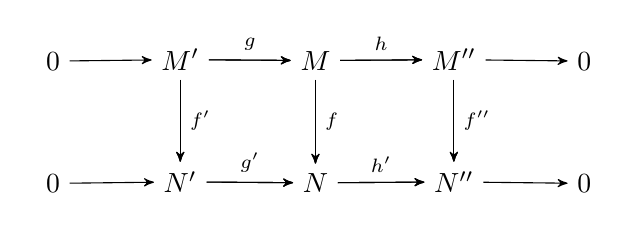
\begin{tikzpicture}
	  \matrix (m) [matrix of math nodes, row sep=3em, column sep=3em]
	    { 0 & M'  & M  & M''  & 0 \\
	      0 & N' & N & N'' & 0 \\ };
	  { [start chain] \chainin (m-1-1);
	    \chainin (m-1-2);
	    { [start branch=A] \chainin (m-2-2)
	        [join={node[right] {$\scriptstyle f'$}}];}
	    \chainin (m-1-3) [join={node[above] {$\scriptstyle g$}}];
	    { [start branch=B] \chainin (m-2-3)
	        [join={node[right] {$\scriptstyle f$}}];}
	    \chainin (m-1-4) [join={node[above] {$\scriptstyle h$}}];
	    { [start branch=C] \chainin (m-2-4)
	        [join={node[right] {$\scriptstyle f''$}}];}
	    \chainin (m-1-5); }
	  { [start chain] \chainin (m-2-1);
	    \chainin (m-2-2);
	    \chainin (m-2-3) [join={node[above] {$\scriptstyle g'$}}];
	    \chainin (m-2-4) [join={node[above] {$\scriptstyle h'$}}];
	    \chainin (m-2-5); }
	\end{tikzpicture}
	\end{center}

be a commutative diagram of $R$-modules and homomorphisms, with the rows exact. Then there exists a sequence $$0 \rightarrow \ker(f') \xrightarrow{\overline u} \ker(f) \xrightarrow{\overline v} \ker (f'') \xrightarrow d \coker(f') \xrightarrow {\overline u'} \coker (f) \xrightarrow{\overline v'} \coker(f'') \rightarrow 0$$ in which $\overline u$, $\overline v$ are restrictions of $u, v$, and $\overline u', \overline v'$ are induced by $u', v'$.\\

	\begin{proof}
	We consider: 	
	\begin{center}
	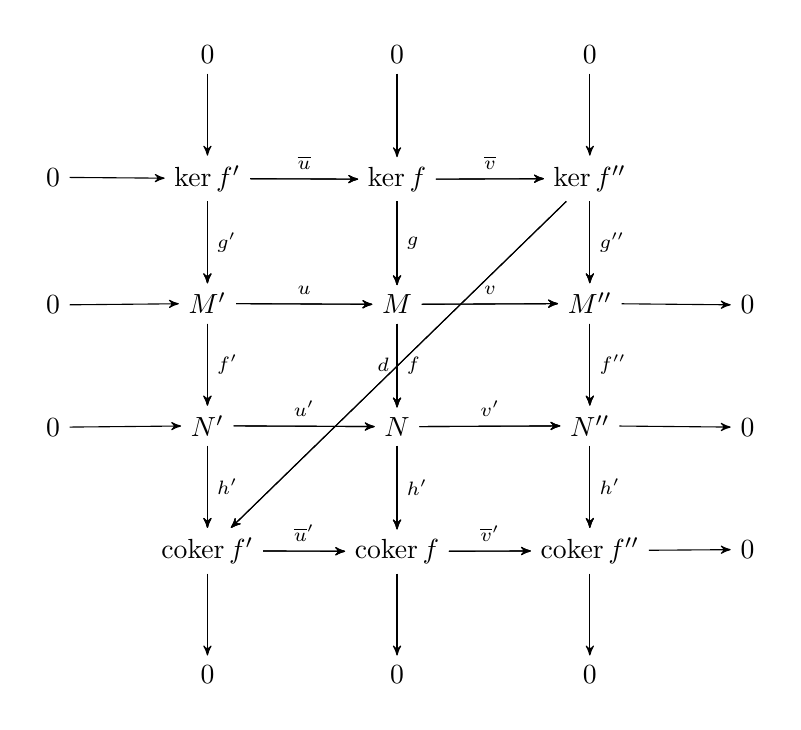
\begin{tikzpicture}

	\matrix (m) [matrix of math nodes, row sep=3em, column sep=3em]
	  {  & 0  & 0 & 0   & \\
	   0 & \ker f' & \ker f & \ker f'' & \\
	   0 & M' & M & M'' & 0\\
	   0 & N' & N & N'' & 0\\
	   & \coker f' & \coker f & \coker f'' & 0\\
	     & 0  & 0 & 0   & \\};
	{ [start chain] \chainin (m-1-2); { [start branch = A] \chainin (m-2-2); } }
	{ [start chain] \chainin (m-1-3); { [start branch = B] \chainin (m-2-3); } }
	{ [start chain] \chainin (m-1-4); { [start branch = C] \chainin (m-2-4); } }
	{ [start chain] 
		\chainin (m-2-1);
		\chainin (m-2-2); 
			{ [start branch = D] \chainin (m-3-2) [join = {node[right] {$\scriptstyle g'$}}]; } 
		\chainin (m-2-3) [join = {node[above] {$\scriptstyle \overline u$}}];
			{ [start branch = E] \chainin (m-3-3) [join = {node[right] {$\scriptstyle g$}}]; }
		\chainin (m-2-4) [join = {node[above] {$\scriptstyle \overline v$}}];
			{ [start branch = F] \chainin (m-3-4) [join = {node[right] {$\scriptstyle g''$}}]; }
		\chainin (m-5-2) [join = {node[left] {$\scriptstyle d$}}];
	}
	{ [start chain] 
		\chainin (m-3-1);
		\chainin (m-3-2); 
			{ [start branch = G] \chainin (m-4-2) [join = {node[right] {$\scriptstyle f'$}}]; } 
		\chainin (m-3-3) [join = {node[above] {$\scriptstyle u$}}];
			{ [start branch = H] \chainin (m-4-3) [join = {node[right] {$\scriptstyle f$}}]; }
		\chainin (m-3-4) [join = {node[above] {$\scriptstyle v$}}];
			{ [start branch = I] \chainin (m-4-4) [join = {node[right] {$\scriptstyle f''$}}]; }
		\chainin (m-3-5);
	}
	{ [start chain] 
		\chainin (m-4-1);
		\chainin (m-4-2); 
			{ [start branch = J] \chainin (m-5-2) [join = {node[right] {$\scriptstyle h'$}}]; } 
		\chainin (m-4-3) [join = {node[above] {$\scriptstyle u'$}}];
			{ [start branch = K] \chainin (m-5-3) [join = {node[right] {$\scriptstyle h'$}}]; }
		\chainin (m-4-4) [join = {node[above] {$\scriptstyle v'$}}];
			{ [start branch = L] \chainin (m-5-4) [join = {node[right] {$\scriptstyle h'$}}]; }
		\chainin (m-4-5);
	}	
	{ [start chain] 
		\chainin (m-5-2); 
			{ [start branch = M] \chainin (m-6-2); } 
		\chainin (m-5-3) [join = {node[above] {$\scriptstyle \overline u'$}}];
			{ [start branch = N] \chainin (m-6-3); }
		\chainin (m-5-4) [join = {node[above] {$\scriptstyle \overline v'$}}];
			{ [start branch = O] \chainin (m-6-4); }
		\chainin (m-5-5);
	}	
	\end{tikzpicture}
	\end{center}

	By Rotman Exercise 2.32, we have that $\im \overline u = \ker \overline v$ and $\im \overline u' = \ker \overline v'$. It is left for us to first define $d$ and then show that $\im \overline v = \ker d$ and $\im d = \ker \overline u'$.
	\end{proof}




\end{document}
